\section{Results}
Loss function expectedly shows convergence and decreases quickly.
\begin{minipage}{\linewidth}
    \centering% 
    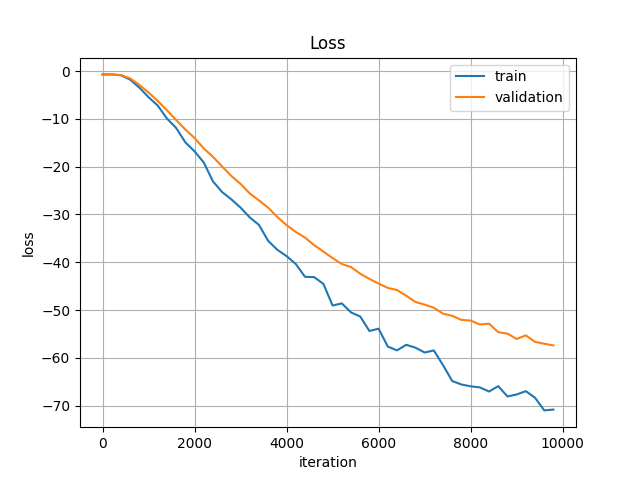
\includegraphics[scale=0.35]{assets/loss.png}% 
    \figcaption{Loss (BPR)}% 
    \label{fig:res:loss}% 

    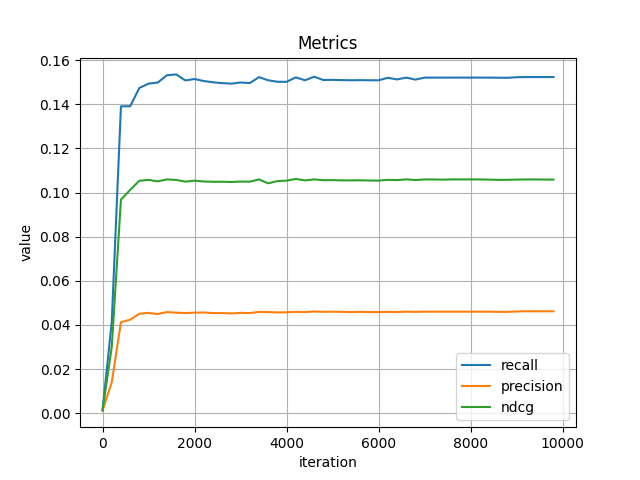
\includegraphics[scale=0.35]{assets/metrics.png}% 
    \figcaption{Metrics}% 
    \label{fig:res:metrics}% 

\end{minipage}

However, loss function is negative, which can be considered pretty strange. I
believe, that the issue is with the implementation, but not sure where. It is
fine, since the general behaviour of loss is as expected.

Metrics behave pretty good as well. All three metrics converge to the certain
value within some time interval.

Even though the overall loss continuous to degrease on both train and
validation, metrics do not tend to further increase, so there is no point in
continuing the training. Without any meaningful changes to the model, it would
be difficult to improve the results.